\section{The Master Method}
\label{sec:the_master_method}

\begin{frame}
	\frametitle{The master method}
	\framesubtitle{Not in the book!}
	\begin{center}
		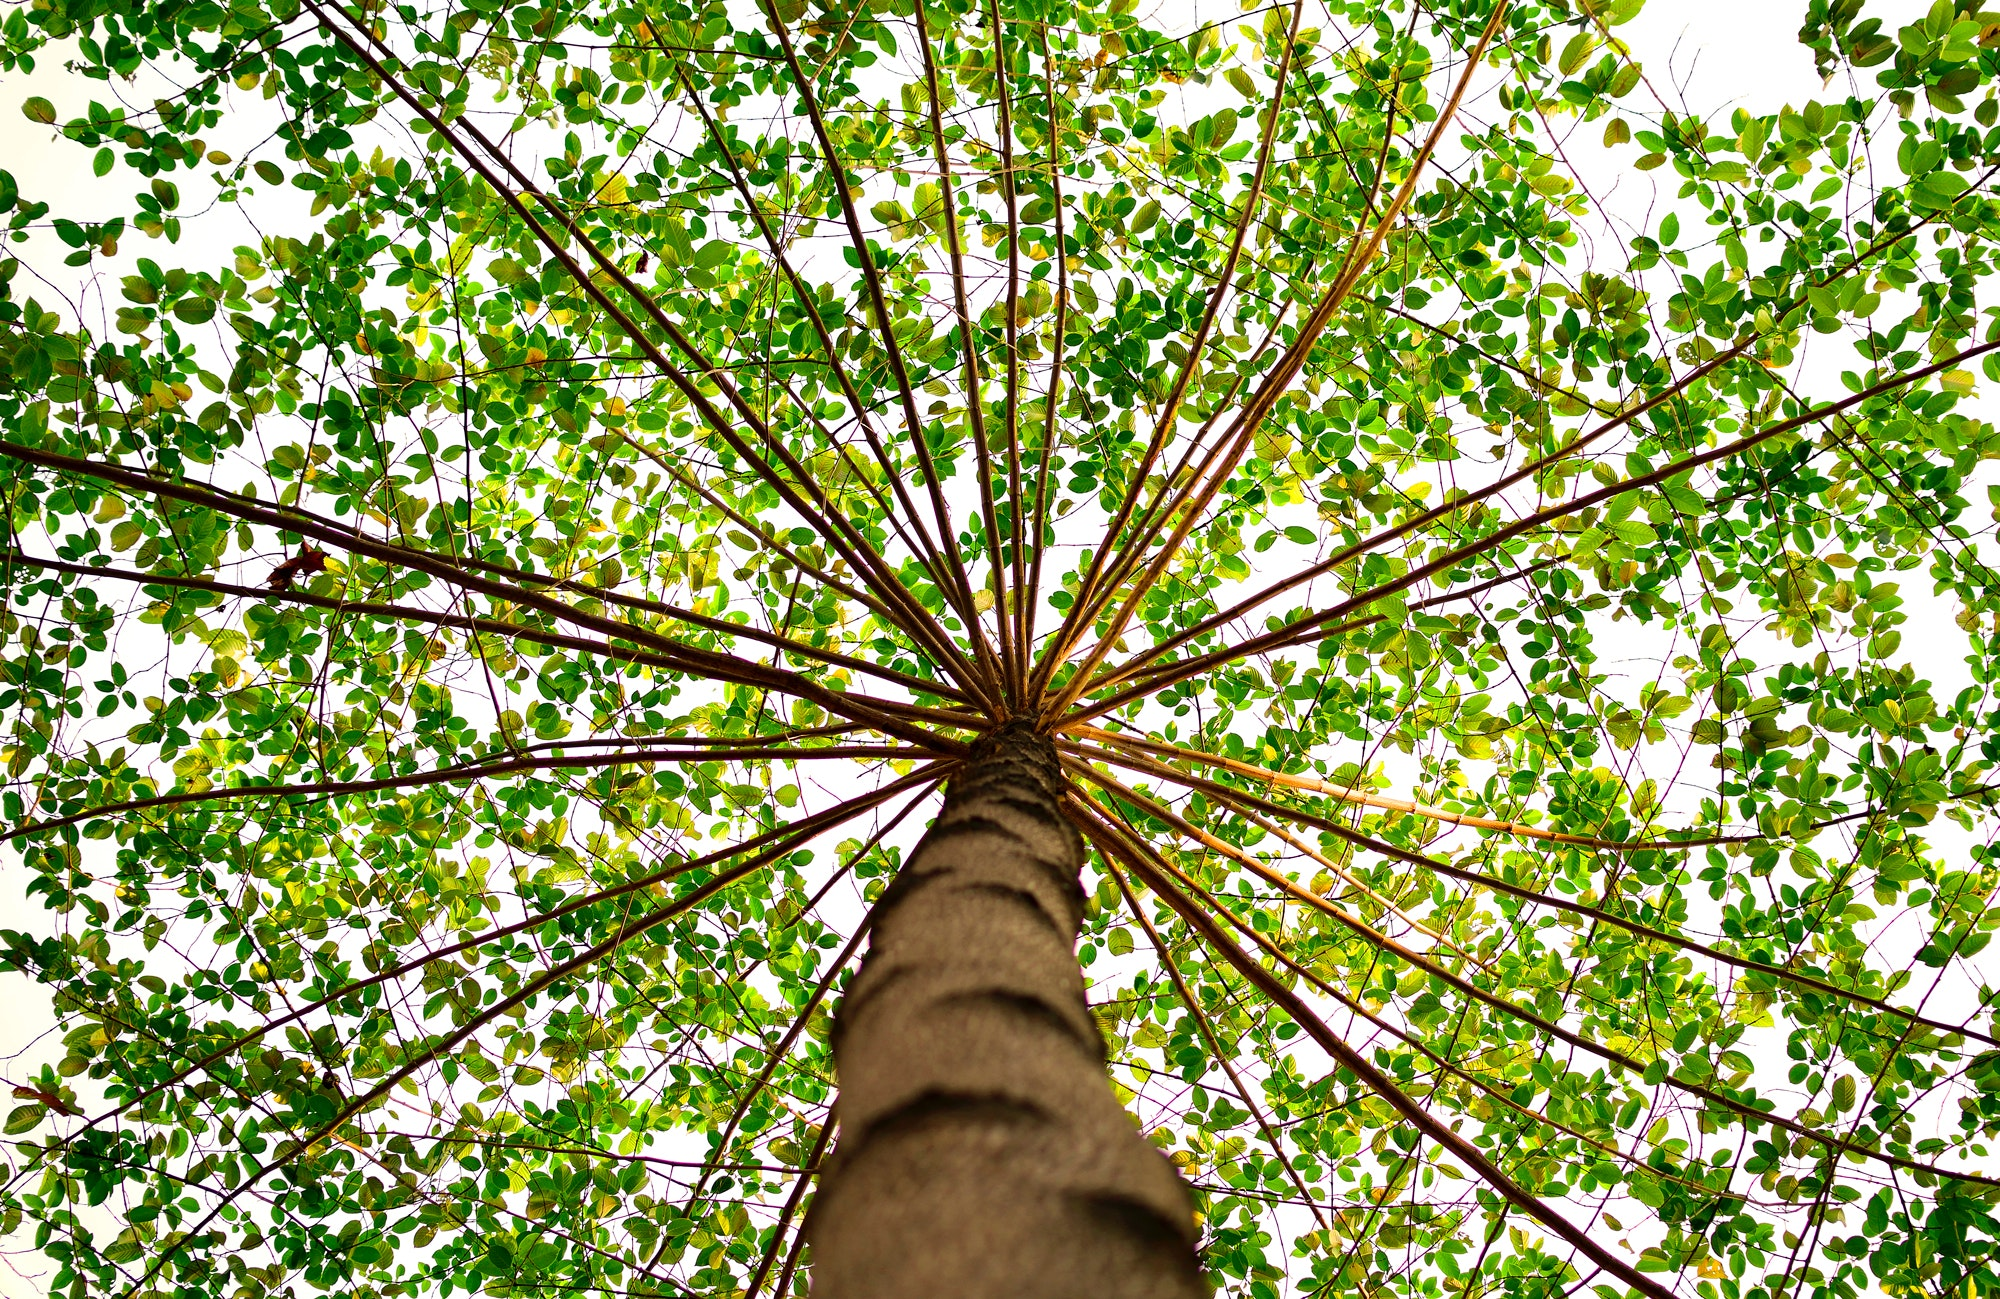
\includegraphics[width=0.7\textwidth]{figures/tree.jpg}\\
		\hspace*{15pt}\hbox{\scriptsize Image By:\thinspace{\itshape Lerkrat Tangsri}}
		%https://www.pexels.com/photo/wood-light-nature-forest-91153/
	\end{center}
	\pnote{We take a break from the problem for a bit}
\end{frame}

\begin{frame}
	\frametitle{General recursion tree}
	\begin{block}{Recurrence equation}
		For $a\geq 1$	and $b \geq 2$:\\
		$T(n) = \begin{cases}
			\Theta(1) & \text{if } n=1\\
			aT(n/b) + f(n) & \text{else}
		\end{cases}$
	\end{block}		
	\vspace{-5pt}
	\begin{figure}[htpb]
	\begin{center}
		\begin{tikzpicture}[scale=0.45, transform shape]

			\foreach \x in {0}{
				\node[draw, rectangle, fill=gray!10, minimum size = 0.4] (a\x) at (\x*8,8) {$T(n)$};
				\foreach \y in {0,...,2}{
					\node[draw,rectangle, fill=gray!10, minimum size =0.4] (b\y) at (-4+\x*8+\y*4,6) {$T(n/b)$};
					\draw (a\x) -- (b\y);
					\draw[dotted] (-6,7) -- node[fill=white] {$a$ calls} (6,7);
					\only<2->{
						\foreach \z in {0,...,2}{
							\ifthenelse{\y = 1}{
								\node[] (c\z) at (-1.5+\z*1.5,4.8) { };
								\draw[dashed] (b\y) -- (c\z);
								}{
								\node[draw,rectangle, fill=gray!10, minimum size =0.4] (c\z) at (-6+\x*8+\y*4+\z*2,4) {$T(n/b^2)$};
								\draw (b\y) -- (c\z);
								\foreach \a in {0,...,2}{
									\node[] (d\a) at (-6.5+\x*8+\y*4+\z*2+\a*0.5,2) { };
									\draw[dashed] (c\z) -- (d\a);
								}
							}
							\draw[dotted] (-5.5+\x*8+\y*4,5) -- node[fill=white] {$a$ calls} (-6+\x*8+\y*4+3.5,5);
						}
					}
				}
			}
			\node at (14, 0) { };

			\only<3->{
				\draw[fill=blue!60] (-8,2) rectangle node {$T(n/b^k)$} (7,3);
			}

			\only<4->{
				\foreach \x in {0,...,4}{
					\node[] (b\x) at (-7+\x*3,2) { };
					\node[draw, rectangle, fill=gray!10, minimum size = 0.4] (a\x) at (-8+\x*3,1) {$T(1)$};
					\draw[dotted] (b\x) -- (a\x);
				}

				\foreach \x in {0,...,4}{
					\node[] (b\x) at (-7+\x*3,2) { };
					\node[] (a\x) at (-7+\x*3,1) { };
					\draw[dotted] (b\x) -- (a\x);
				}

				\foreach \x in {0,...,4}{
					\node[] (b\x) at (-7+\x*3,2) { };
					\node[draw, rectangle, fill=gray!10, minimum size = 0.4] (a\x) at (-6+\x*3,1) {$T(1)$};
					\draw[dotted] (b\x) -- (a\x);
				}
			}

			\only<5->{
				\node at (9,9) {\Large Amount of nodes $\cdot$ combining};
				\node at (9,7.9) {\Large $1 \cdot f(n)$};
				\node at (9,5.9) {\Large $a \cdot f(n/b)$};
				\node at (9,3.9) {\Large $a^2 \cdot f(n/b^2)$};
			}

			\only<6->{
				\node at (9,2.3) {\Large $a^k \cdot f(n/b^k)$};
				\node at (9,1.2) {\Large $a^{\log_b n } \cdot f(1)$};
			}

			\only<7->{
				\draw (7,0.5) -- (11,0.5) node[anchor = west] {\Large $+$};
				\node at (9,-0.2) {\Large $\sum\limits_{i=0}^{log_b n} a^i \cdot f(\dfrac{n}{b^i})$};
			}

			\only<8->{
				\node[anchor=west] at (-7, -0.2) {\Large Total time spent in the leaves: $\Theta(a^{\log_b n}) = \Theta(n^{\log_b a})$.};
			}

			\only<9->{
				\node[red, anchor=west] at (5, -0.2) {\Large $\leq, =, \geq$};
				\node[red, anchor=west] at (4.7, -1.2) {\Large Which is it?};
			}

		\end{tikzpicture}
	\end{center}
\end{figure}

\end{frame}

\begin{frame}
	\frametitle{The master method}
	\begin{columns}[t]
		\column{0.455\textwidth}
	\begin{block}{Recurrence equation}
		For $a\geq 1$	and $b \geq 2$:\\
		$T(n) = \begin{cases}
			\Theta(1) & \text{if } n=1\\
			aT(n/b) + f(n) & \text{else}
		\end{cases}$
	\end{block}		
			
		\column{0.455\textwidth}

	\begin{answerblock}{From the tree}
		$T(n) = \Theta(n^{\log_b a}) + \sum\limits_{i=0}^{\log_b n} a^i\cdot f(\dfrac{n}{b^i})$, where:
		\begin{itemize}
			\item the first term represents the work in the leaves.
			\item the second term represents the work in combining the results.
		\end{itemize}
	\end{answerblock}
			
	\end{columns}

	\pause
	\hfill\\
	There are three common cases. The running time is: 
	\begin{enumerate}
		\item	dominated by \alert{the leaves}.
		\item	\alert{evenly distributed} throughout the tree.
		\item	dominated by \alert{the root}.
	\end{enumerate}

\end{frame}

\begin{frame}
	\frametitle{One method to rule them all}

	\begin{overlayarea}{\textwidth}{1.2\textheight}
		\begin{problemblock}{The recurrence equation}
			\scriptsize
			A recurrence equation in the form: $T(n) = a T(n/b) + f(n)$.
		\end{problemblock}
		
		\begin{answerblock}{The solution}
				\scriptsize
			Three common cases:
			\begin{enumerate}
				\item	dominated by \alert{the leaves}. \hfill\\
					If $f(n)$ is $O(n^{\log_b a - \epsilon})$, then $T(n)$ is $\Theta(n^{\log_b a})$. {\small\hfill for some $\epsilon > 0$}
				\item<2->	\alert{evenly distributed} throughout the tree.\hfill\\
					If $f(n)$ is $\Theta(n^{\log_b a})$, then $T(n)$ is $\Theta(n^{\log_b a} \log n)$. 
				\item<3->	dominated by \alert{the root}.\hfill\\
					If $f(n)$ is $\Omega(n^{\log_b a + \epsilon})$, then $T(n)$ is $ \Theta(f(n))$. {\small\hfill for some $\epsilon > 0$}
			\end{enumerate}	
		\end{answerblock}
		\only<3->{
			\begin{block}{Case 3 has a special requirements}
				\small
				Check the regularity condition: $a f(n/b) \leq c f(n)$. For some $c < 1$.\\
				Hint: Polynomials always satisfy this condition.
			\end{block}	
		}
	\end{overlayarea}
\end{frame}

\begin{frame}
	\frametitle{Let's do some examples}
	\framesubtitle{XKCD: \url{https://xkcd.com/189/}}

	\begin{center}
		
\includegraphics[width=0.7\textwidth]{figures/exercise.png}
	\end{center}
\end{frame}

%\begin{frame}
%	\frametitle{Example 2 - Merge sort}
%	\begin{overlayarea}{\textwidth}{\textheight}
%		\begin{block}{The method}
%			\small
%			\begin{itemize}
%				\item Identify $a$, $b$, $f(n)$ from a given recurrence equation.
%				\item Determine $n^{\log_b a}$.
%				\item Compare $n^{\log_b a}$ and $f(n)$.
%				\item Determine the right case from the master method and apply. 
%			\end{itemize}
%		\end{block}	
%		\only<2>{
%			\begin{problemblock}{Example 2 - Merge sort}
%				\small
%				$T(n) = 2 T(n/2) + \Theta(n)$	\\
%				Which part of the algorithm uses strictly more time?
%				\begin{enumerate}[A.]
%					\item Work in the leaves: $n^{\log_b a}$.
%					\item Work in the root node: $f(n)$.
%					\item Evenly spread throughout the tree.
%					\item We cannot apply the master method.
%				\end{enumerate}
%			\end{problemblock}
%		}
%		\only<3>{
%			\begin{answerblock}{Example 2 - Merge sort}
%				\small
%				$T(n) = 2 T(n/2) + \Theta(n)$	\\
%				$a = 2, b =2, n^{\log_b a} = n^{\log_2 2} = n$\\
%				$f(n)$ is $\Theta(n)$\\
%				So case 2 of the master method, thus $T(n)$ is $\Theta(n^{\log_2 2} \log n) =\Theta(n \log n)$.
%			\end{answerblock}
%		}
%	\end{overlayarea}
%\end{frame}

\begin{frame}
	\frametitle{Example 1 - Binary Search}
	\framesubtitle{From last week}
	\begin{overlayarea}{\textwidth}{\textheight}
		\begin{columns}
			\column{0.455\textwidth}
				
		\begin{algorithmic}
			\scriptsize
			\Function{Binary-Search}{A,p,q,r,s}
			\State $q \gets (p+r)/2$
			\If{$p > r$}
			\State \Return false
			\ElsIf{$a[q] = s$}
			\State \Return $q$
			\ElsIf{$a[q] > s$}
			\State \Return \Call{Binary-Search}{a,p,q-1,s}
			\Else
			\State \Return \Call{Binary-Search}{a,q+1,r,s}
			\EndIf
			\EndFunction
		\end{algorithmic}
			\column{0.455\textwidth}
				
		\only<3->{
			\begin{problemblock}{Example 1 - Binary search}
				Which part of the algorithm uses strictly more time?
				\begin{enumerate}[A.]
					\small
					\item Work in the leaves: $n^{\log_b a}$.
					\item Work in the root node: $f(n)$.
					\item Evenly spread throughout the tree.
					\item We cannot apply the master method.
				\end{enumerate}
			\end{problemblock}
		}
		\only<2>{
			\begin{problemblock}{Example 1 - Binary search}
				So what is the recurrence equation again?
					\begin{enumerate}[A.]
						\item $T(n) = T(n/2) + c$
						\item $T(n) = T(n/2) + n$
						\item $T(n) = 2T(n/2) + c$
						\item $T(n) = 2T(n/2) + n$
						\item $T(n) = 2T(n/2) + n\log n$
						\item I don't know.
					\end{enumerate}
			\end{problemblock}
		}
		\end{columns}
		\only<4>{
			\begin{answerblock}{Example 1 - Binary search}
				\small
				$T(n) = T(n/2) + \Theta(1)$	\\
				$a = 1, b =2, n^{\log_b a} = n^{\log_2 1} = n^0 = 1$\\
				$f(n)$ is $\Theta(1)$\\
				So case 2 of the master method, thus $T(n)$ is $\Theta(n^{\log_2 1} \log n) =\Theta(\log n)$.
			\end{answerblock}
		}
	\end{overlayarea}
\end{frame}

\begin{frame}
	\frametitle{Example 2 - 9 \st{rings} calls}
	\begin{overlayarea}{\textwidth}{\textheight}
		\begin{problemblock}{Example 2}
			\small
			$T(n) = 9 T(n/3) + n$	\\
			\only<1>{
				Which part of the algorithm uses strictly more time?
				\begin{enumerate}[A.]
					\item Work in the leaves: $n^{\log_b a}$.
					\item Work in the root node: $f(n)$.
					\item Evenly spread throughout the tree.
					\item We cannot apply the master method.
				\end{enumerate}
			}
		\end{problemblock}
		\only<2>{
			\begin{answerblock}{Example 2}
				\small
				$a = 9, b =3, n^{\log_b a} = n^{\log_3 9} = n^2$\\
				$f(n)$ is $\Theta(n)$\\
				So case 1 of the master method (most work is in the leaves), \\
				thus $T(n)$ is $\Theta(n^{\log_9 3}) =\Theta(n^2)$.
			\end{answerblock}
		}
	\end{overlayarea}
\end{frame}

\begin{frame}
	\frametitle{Example 3 - Worse binary recursion}
	\begin{overlayarea}{\textwidth}{\textheight}
		\begin{problemblock}{Example 3 - Worse binary recursion}
			$T(n) = T(n/2) + n$
			\only<1>{
				So what is the run time?
				\begin{multicols}{2}
					\begin{enumerate}[A.]
						\item $T(n) $ is $O(n)$.
						\item $T(n) $ is $O(n \log n)$.
						\item $T(n) $ is $O(n^2)$.
						\item $T(n) $ is $O(n^2 \log n)$.
						\item $T(n) $ is $O(n^3)$.
						\item I don't know.
					\end{enumerate}
				\end{multicols}
			}
		\end{problemblock}
		\only<2->{
			\begin{answerblock}{Example 3}
				\small
				$T(n) = T(n/2) + \Theta(n)$	\\
				$a = 1, b =2, n^{\log_b a} = n^{\log_2 1} = n^0 = 1$\\
				$f(n)$ is $\Theta(n)$\\
				So case 3 of the master method, thus $T(n)$ is $\Theta(f(n)) =\Theta(n)$.
				\only<3>{
					\alert{Or is it?}
				}
				\only<4->{
					check regularity condition! Do one of the following:
					\begin{itemize}
						\item observe that $f(n)$ is a polynomial function
						\item observe that $a f(n/b) \leq c f(n)$ for some $c < 1$, in this case: $f(n/2) = n/2 \leq 0.5 n = 0.5
							f(n)$ so for $c = 0.5$
					\end{itemize}
				}
			\end{answerblock}
		}
	\end{overlayarea}
\end{frame}

\begin{frame}
	\frametitle{Example 4 - Multiplying matrices}
	\framesubtitle{From last weeks intermezzo}
	\begin{overlayarea}{\textwidth}{\textheight}
		\begin{problemblock}{Example 4 - Multiplying matrices}
			$T(n) = 7T(n/2) + n^2$
			\only<1>{
				So what is the run time?
				\begin{multicols}{2}
					\begin{enumerate}[A.]
						\item $T(n) $ is $O(n)$.
						\item $T(n) $ is $O(n \log n)$.
						\item $T(n) $ is $O(n^2)$.
						\item $T(n) $ is $O(n^2 \log n)$.
						\item $T(n) $ is $O(n^3)$.
						\item I don't know.
					\end{enumerate}
				\end{multicols}
			}
		\end{problemblock}
		\only<2->{
			\begin{answerblock}{Case ...?}
				\small
				$a = 7, b =2, n^{\log_b a} = n^{\log_2 7} \approx n^{2.81}$\\
				$f(n)$ is $\Theta(n^2)$\\
				\pause
				$f(n)$ is $O(n^{2.81-\epsilon})$ so case 1 (dominated by the leaves)\\
				So $T(n)$ is $\Theta(n^{\log_b a}) \approx \Theta(n^{2.81})$
			\end{answerblock}
		}
	\end{overlayarea}
\end{frame}

